\chapter{Results and Discussion}

\section{System Implementation}
The implemented FlowX platform successfully delivers a comprehensive chatbot development environment. This section presents the key interfaces and functionality of the system, followed by an analysis of its performance and effectiveness. The complete source code for all components is available in the project's GitHub organization\footnote{\url{https://github.com/Chatbot-Builder-Project}}, which contains the following repositories:

\begin{itemize}
    \item \textbf{chatbot-builder-api}: API Gateway for authentication and service orchestration
    \item \textbf{chatbot-builder-client}: Frontend built with React Native
    \item \textbf{chatbot-builder-executor}: LangChain execution service
    \item \textbf{chatbot-builder-infra}: Infrastructure code using Terraform and Kubernetes
    \item \textbf{chatbot-builder-protos}: Protocol Buffer definitions for gRPC communication
\end{itemize}

\section{User Interface and Development Flow}

\subsection{Homepage and Dashboard}
The FlowX platform provides an intuitive entry point for users through its homepage interface (Figure \ref{fig:homepage}).

\begin{figure}[H]
    \centering
    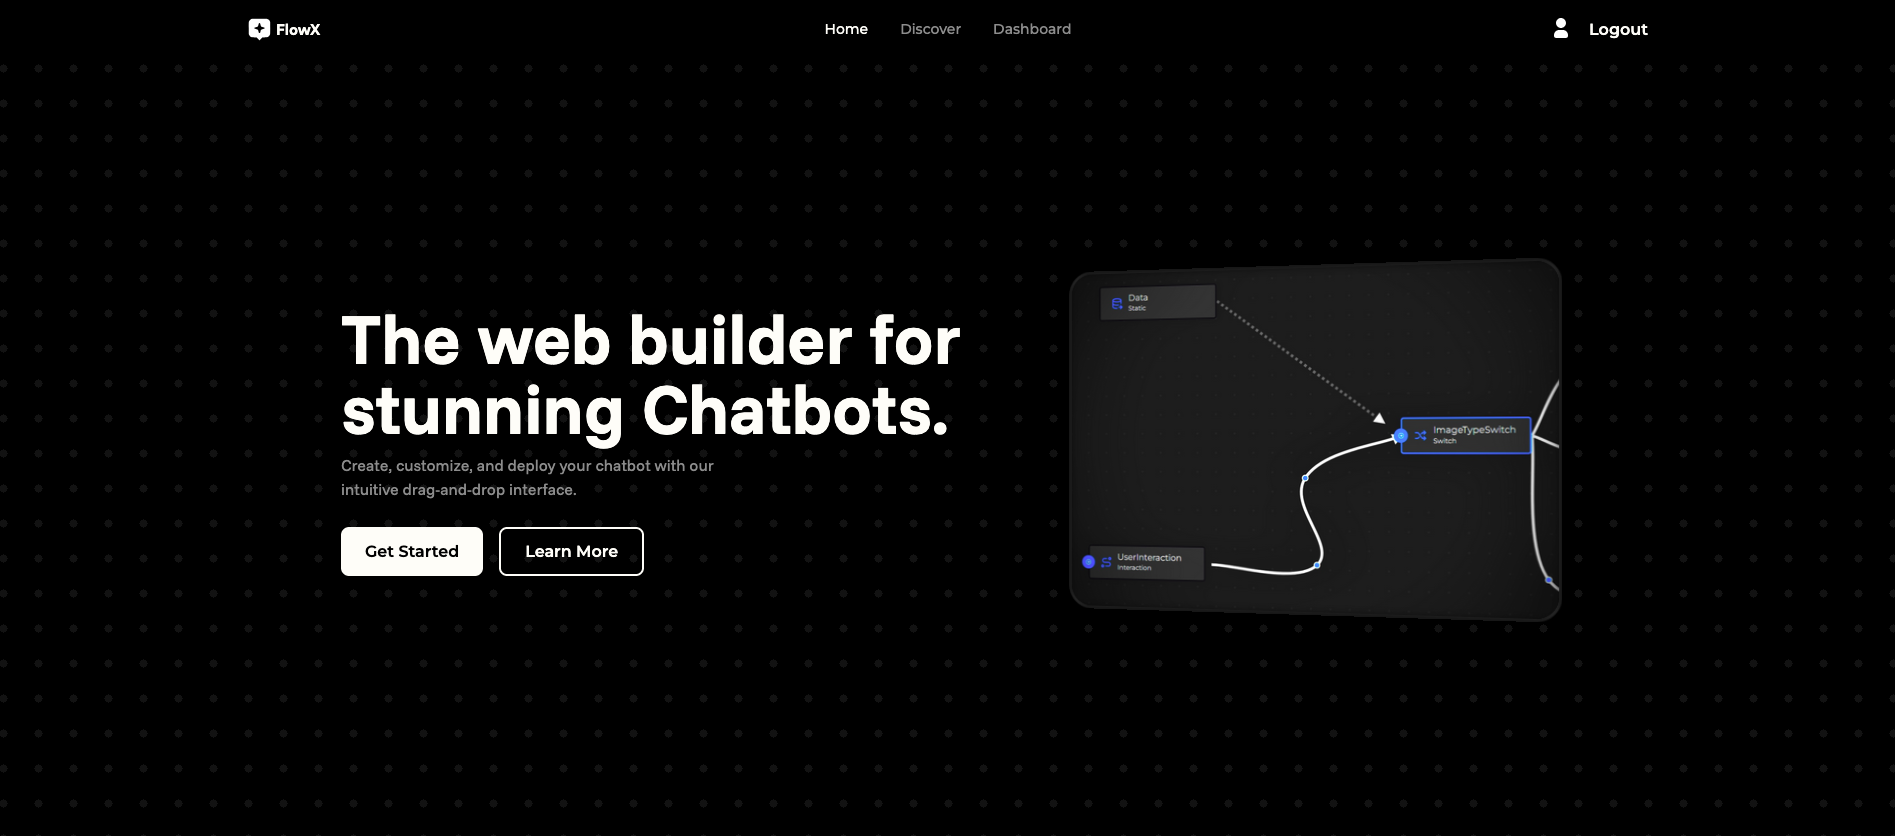
\includegraphics[width=0.95\textwidth]{assets/screenshots/homepage.png}
    \caption{FlowX Platform Homepage}
    \label{fig:homepage}
\end{figure}

\subsection{Workflow Creation}
Users begin by creating a new chatbot project through a streamlined workflow creation process (Figure \ref{fig:create-workflow}).

\begin{figure}[H]
    \centering
    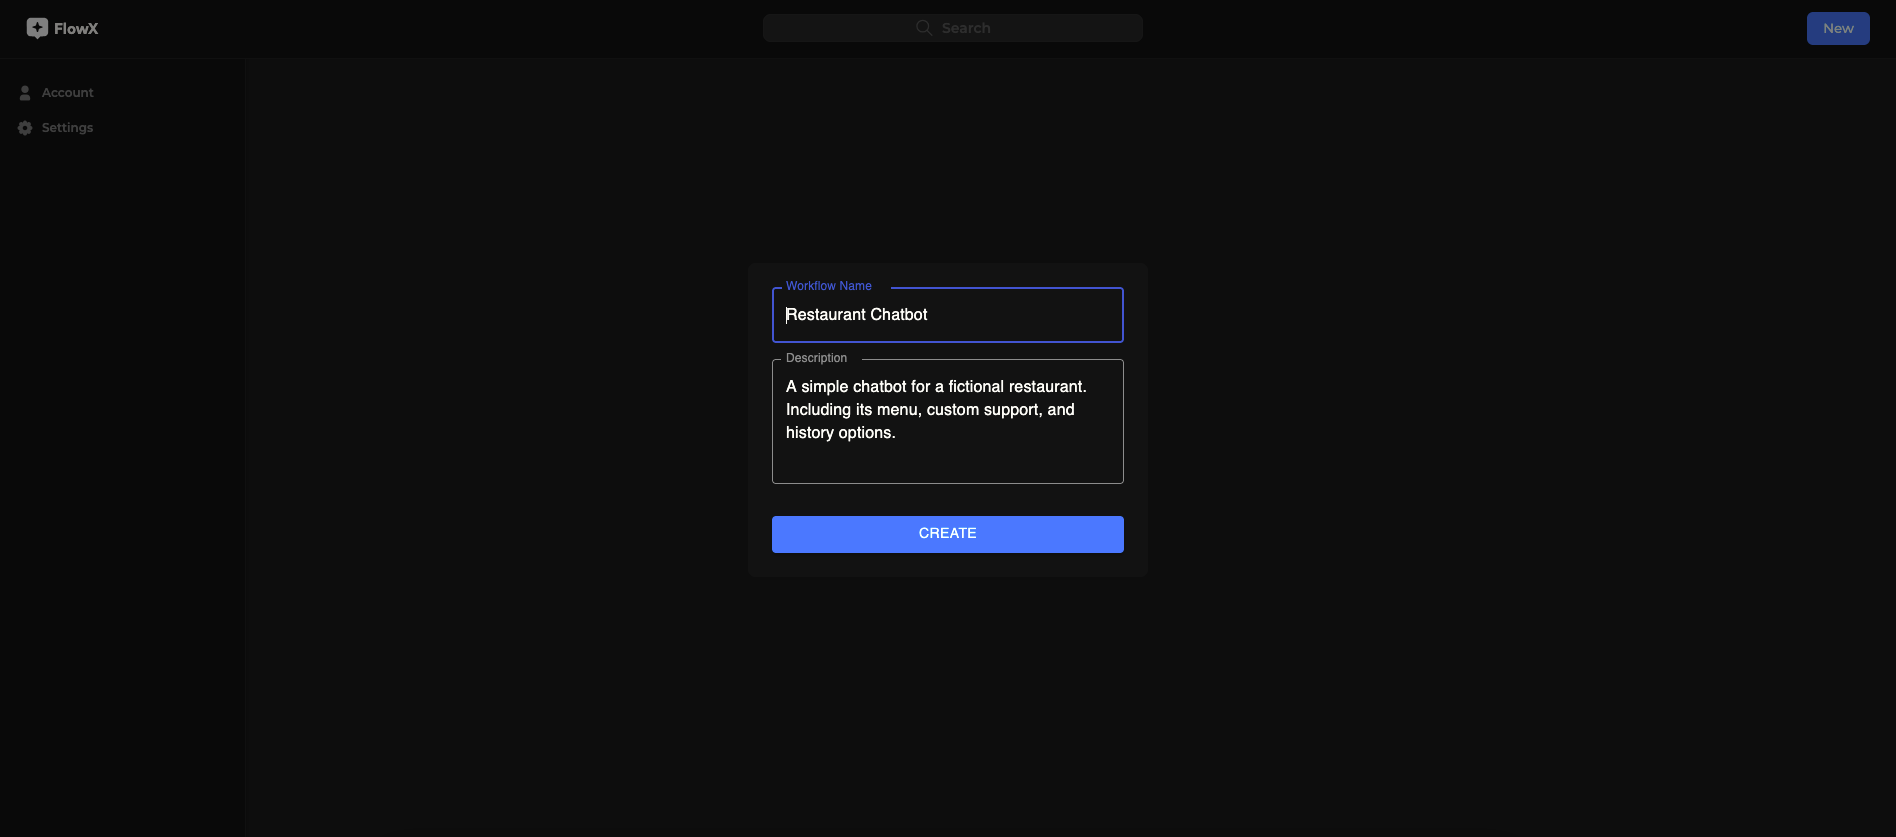
\includegraphics[width=0.95\textwidth]{assets/screenshots/create-workflow.png}
    \caption{Initial Workflow Creation Interface}
    \label{fig:create-workflow}
\end{figure}

\subsection{Workflow Builder}
After creation, users can design their chatbot's conversation logic using the workflow builder. The system provides a simple starter workflow (Figure \ref{fig:workflow1}) that users can build upon. Through the workflow builder's capabilities, users can develop sophisticated conversation patterns, as demonstrated by the complex implementation in Figure \ref{fig:workflow2}.

\begin{figure}[H]
    \centering
    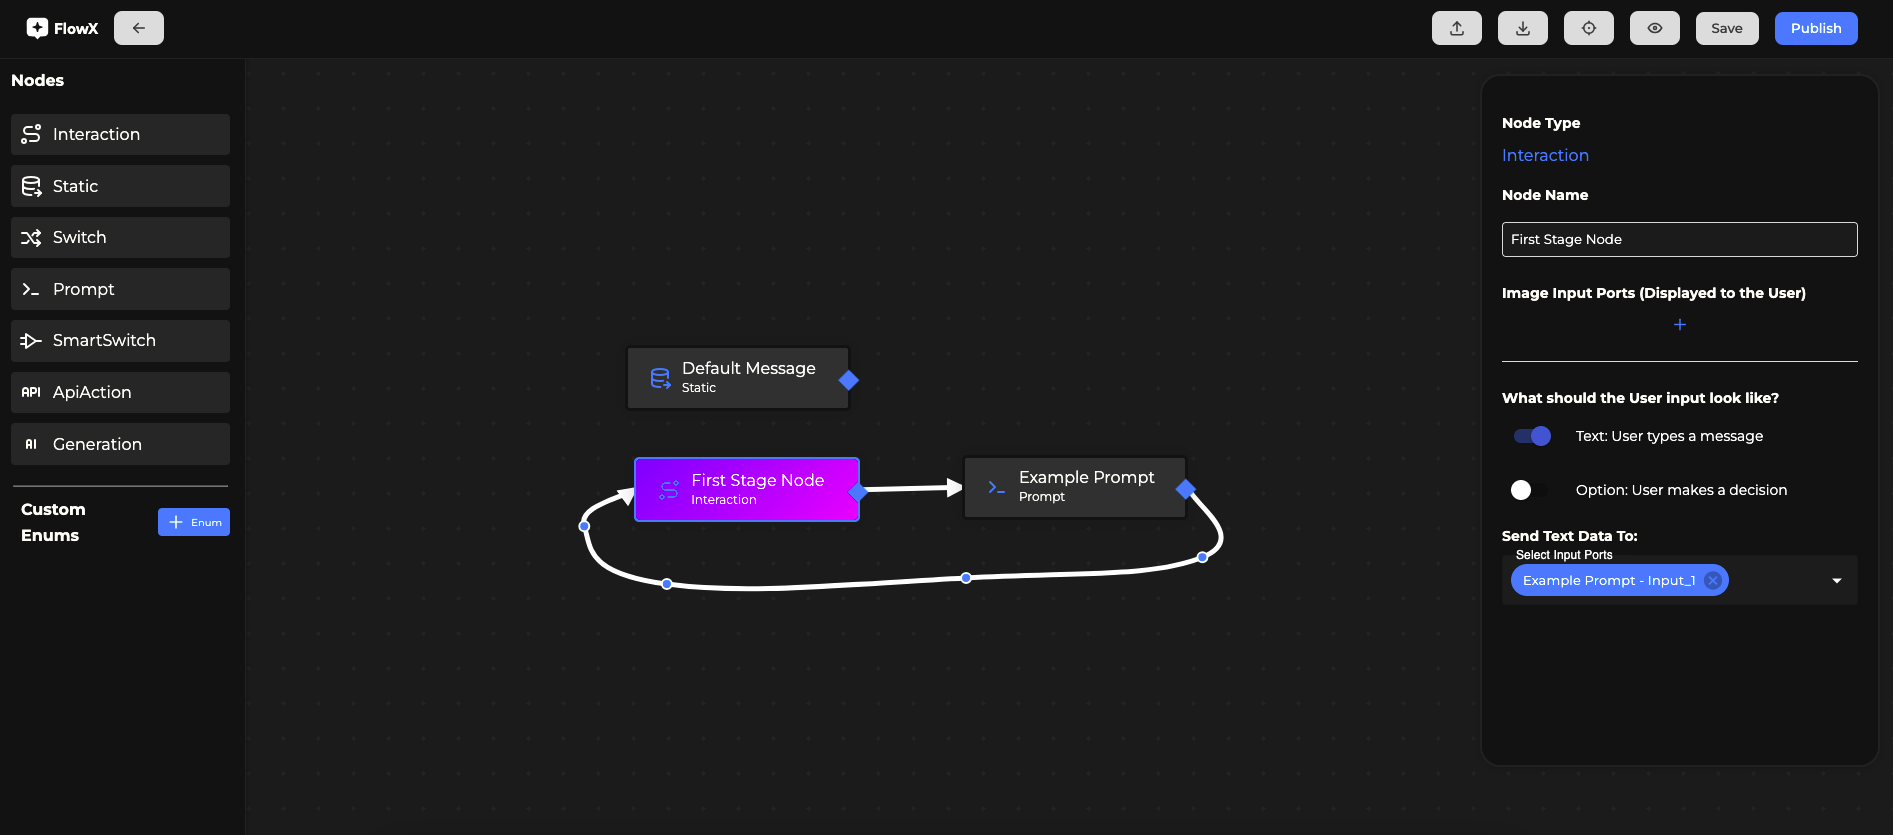
\includegraphics[width=0.95\textwidth]{assets/screenshots/workflow1.png}
    \caption{Initial Default Workflow State}
    \label{fig:workflow1}
\end{figure}

\begin{figure}[H]
    \centering
    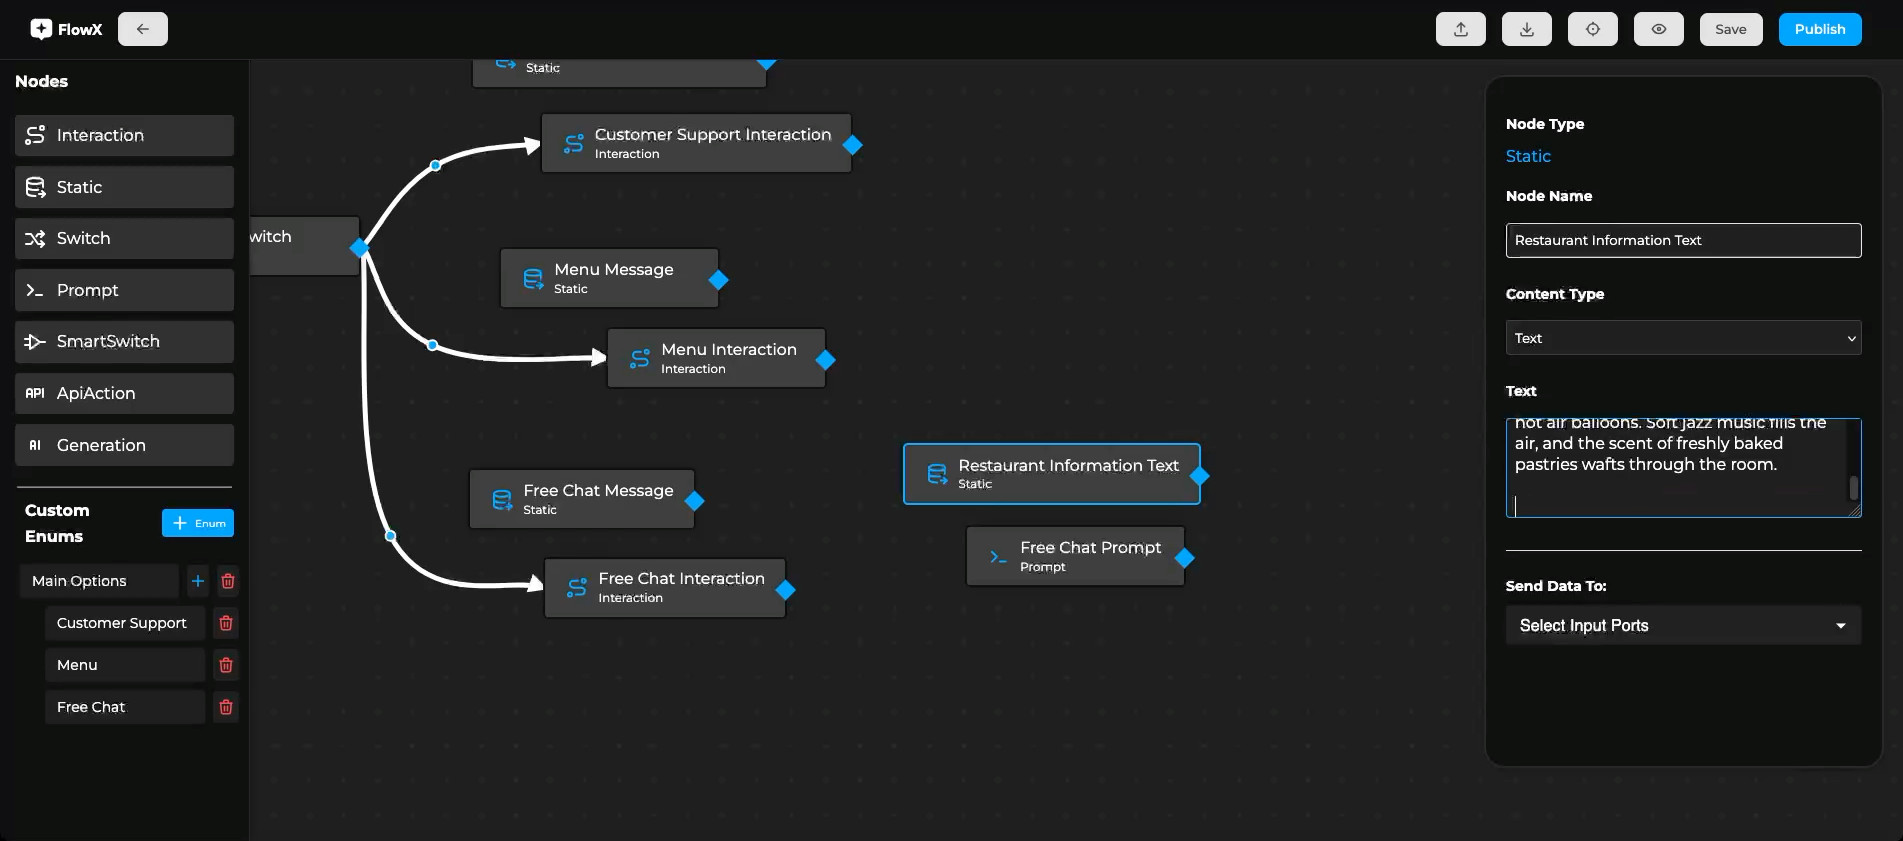
\includegraphics[width=0.95\textwidth]{assets/screenshots/workflow2.jpg}
    \caption{Example of an Advanced Workflow Built Using the Platform}
    \label{fig:workflow2}
\end{figure}

\subsection{Visual Editor}
Once the conversation logic is defined, developers can customize the chatbot's visual appearance using the visual editor (Figure \ref{fig:chatbot-visual-editor}). This interface allows for detailed customization of how the chatbot will appear to end users.

\begin{figure}[H]
    \centering
    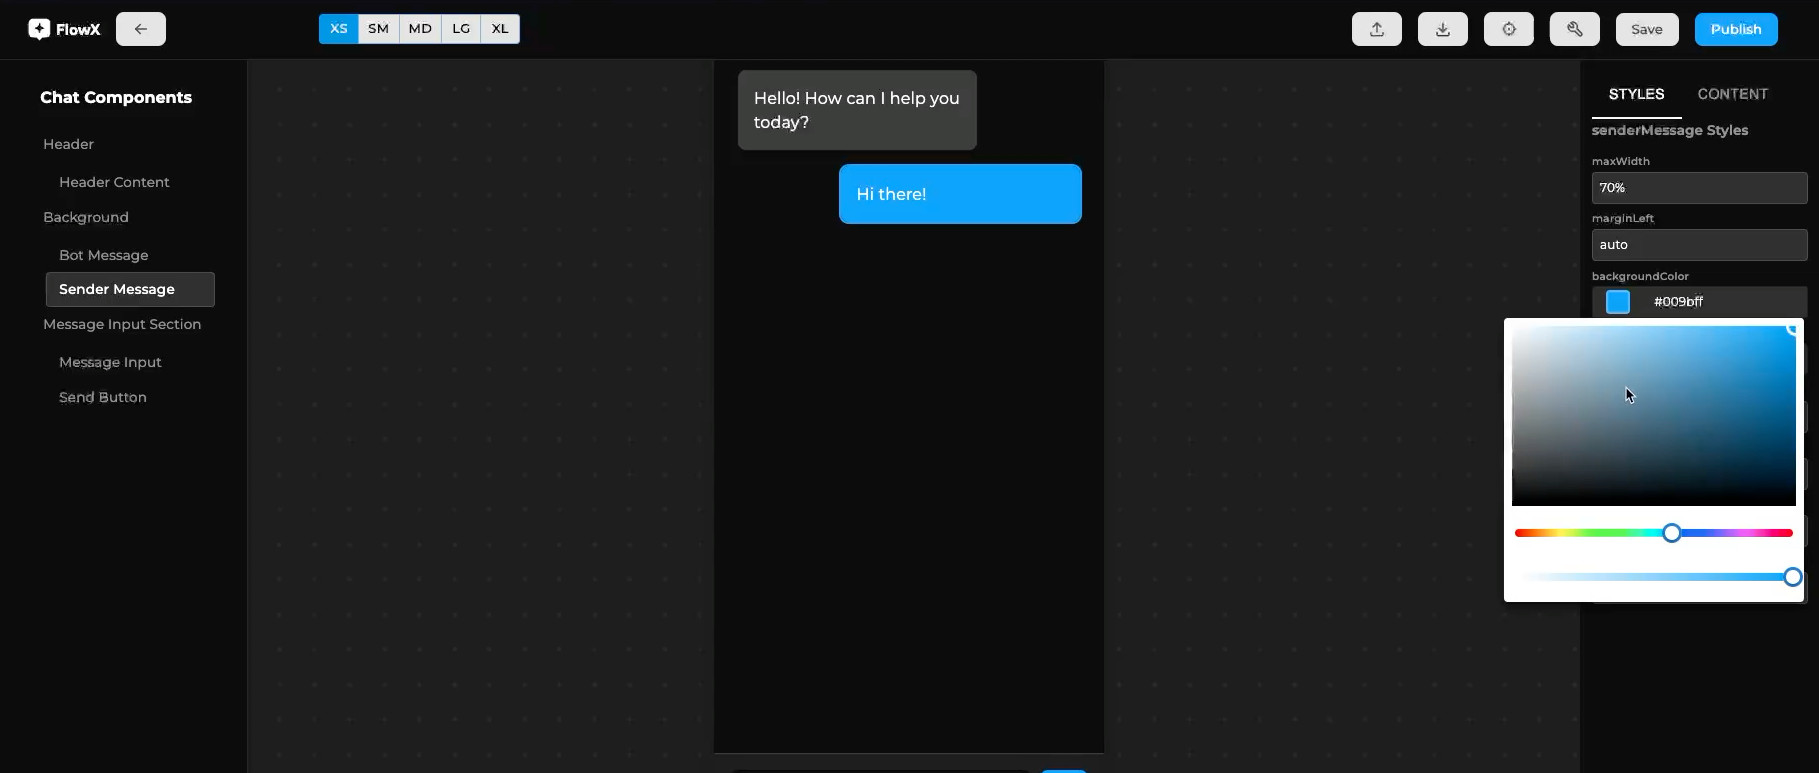
\includegraphics[width=0.95\textwidth]{assets/screenshots/chatbot-visual-editor.jpg}
    \caption{Chatbot Visual Customization Interface}
    \label{fig:chatbot-visual-editor}
\end{figure}

\subsection{Live Testing Interface}
The platform includes a conversation testing interface (Figure \ref{fig:conversation}) that allows developers to validate both their chatbot's logic and visual appearance in real-time.

\begin{figure}[H]
    \centering
    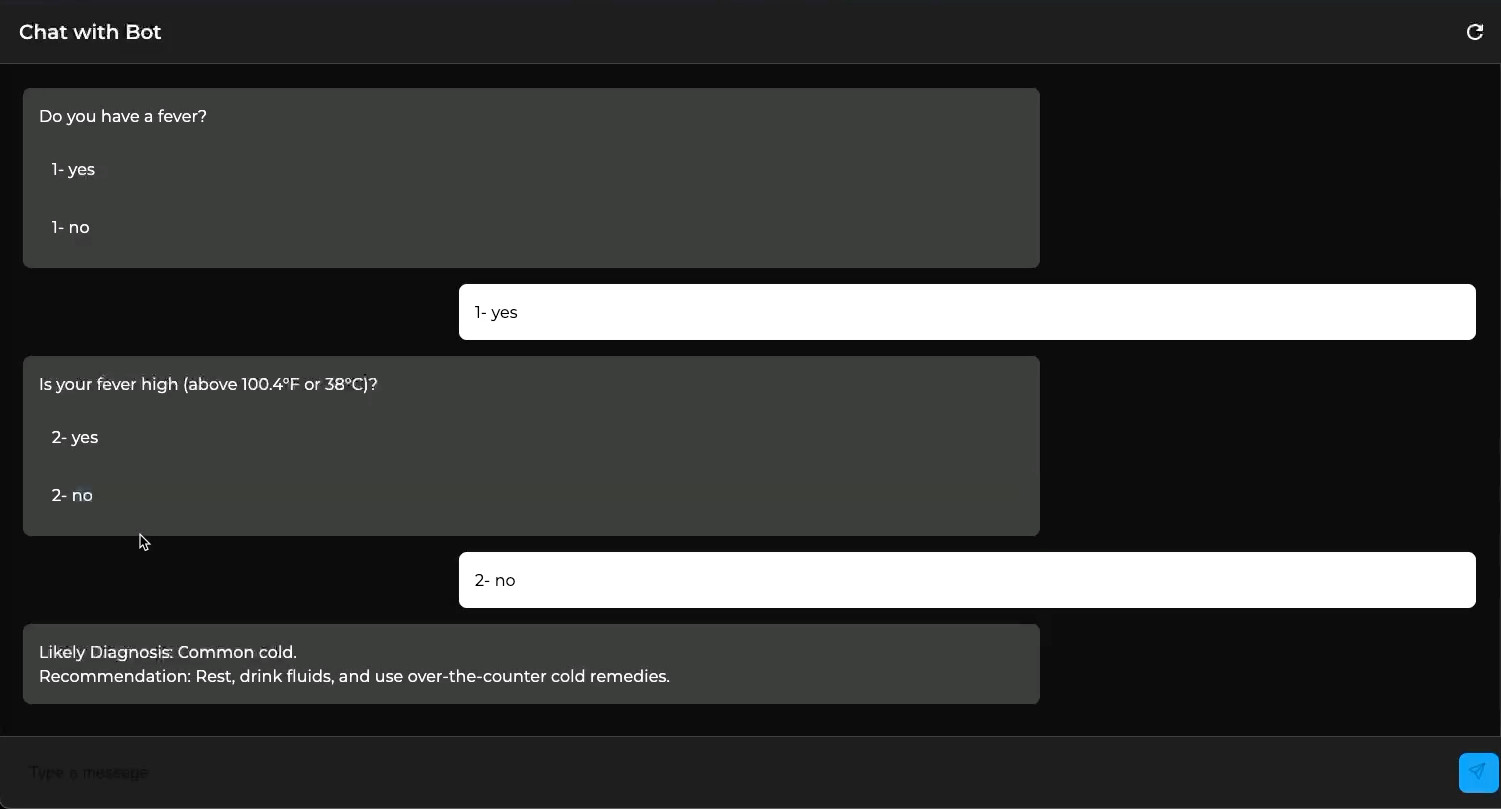
\includegraphics[width=0.95\textwidth]{assets/screenshots/conversation.jpg}
    \caption{Live Conversation Testing Interface}
    \label{fig:conversation}
\end{figure}
